\section{Question 1}

\subsection{What value of $\beta_1$ produces an event-study graph of working hours with something close to a drop in hours of 10\% around the time of birth?}

\bigskip

\paragraph{Economic role of $\beta_1$.}

The parameter $\beta_1$ determines how the presence of a child affects the disutility of labour. In the model

\[
\beta(n_t) = \beta_0 + \beta_1 n_t,
\]

so when a child arrives ($n_t=1$), the marginal disutility of supplying labour increases. Economically, this captures that raising children requires time and effort.

\paragraph{Calibration target.}

\textcite{Kleven2019} show that women's labour supply drops roughly $10\%$ around the first birth.

\begin{figure}[H]
    \centering
    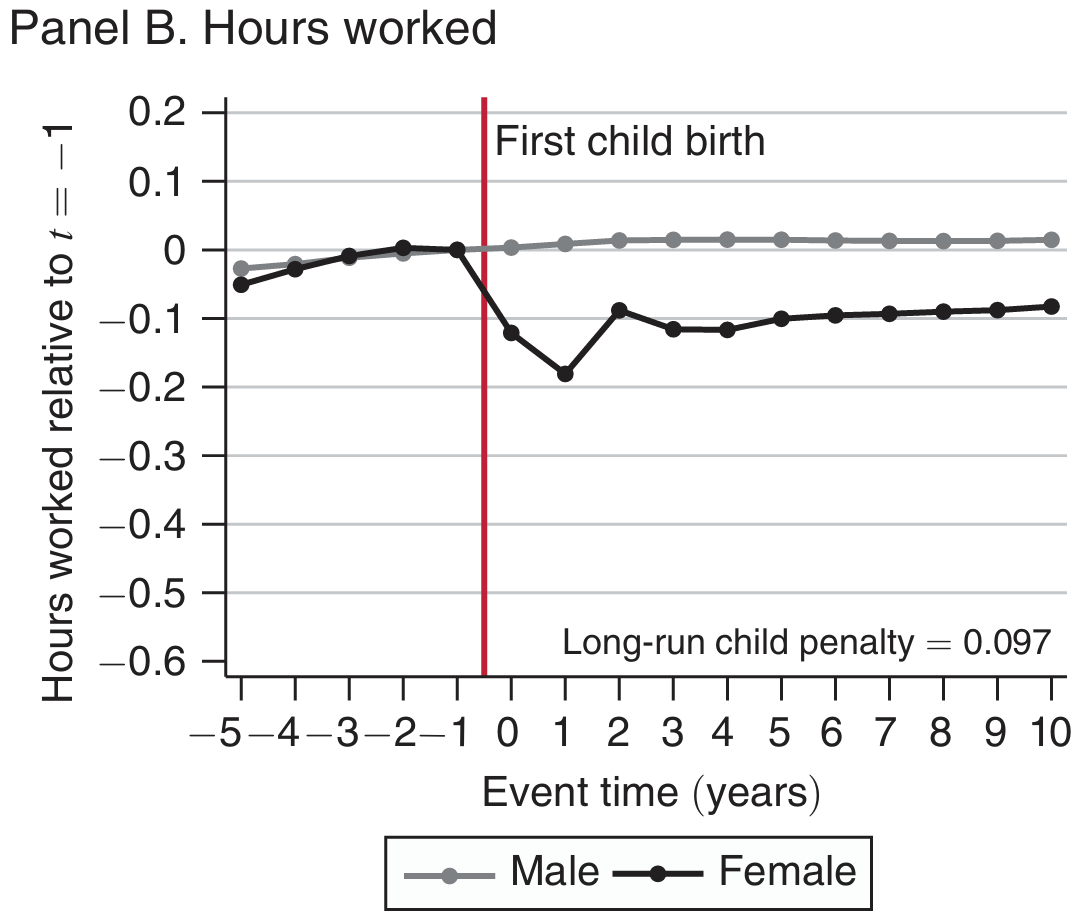
\includegraphics[width=0.5\linewidth]{Billeder/Kleven drop.png}
    \caption{The drop in hours worked, relative to $t-1$ from \cite{Kleven2019}}
    \label{fig:placeholder}
\end{figure}

\paragraph{Calibration procedure.}

We calibrate $\beta_1$ by simulating the model for a candidate value and iteratively adjusting it until the simulated drop in hours matches the $-10\%$ target. For each individual the birth period is identified and an event-study of hours worked around childbirth is constructed.

The calibration problem is

\[
\min_{\beta_1} 
\left(
\textit{Model drop} - (-0.10)
\right)^2,
\]

where \textit{Model drop} denotes the simulated percentage change in hours around childbirth.

Operationally, the procedure proceeds as follows:

\begin{enumerate}
\item Start from an initial guess for $\beta_1$.
\item Solve the model and simulate life-cycle paths.
\item Identify the birth event for each individual.
\item Construct an event-study profile of hours worked.
\item Compute the simulated drop in hours around childbirth.
\item Evaluate the objective function.
\item Update $\beta_1$ and repeat until the simulated drop is close to $-10\%$.
\end{enumerate}

The procedure is implemented using \texttt{minimize} from \texttt{SciPy} with the \texttt{Nelder-Mead} method, an algorithm that iteratively updates candidate parameter values to minimize the objective function.

\paragraph{Calibrated parameter value.}

The algorithm converges to

\[
\beta_1^* = 0.0537,
\]

which produces a simulated decline in hours of approximately $\Delta h \approx -0.10$ around childbirth. The figure title shows the full numerical precision ($\beta_1^* = 0.053672$), which rounds to the reported $0.0537$.

\begin{figure}[H]
    \centering
    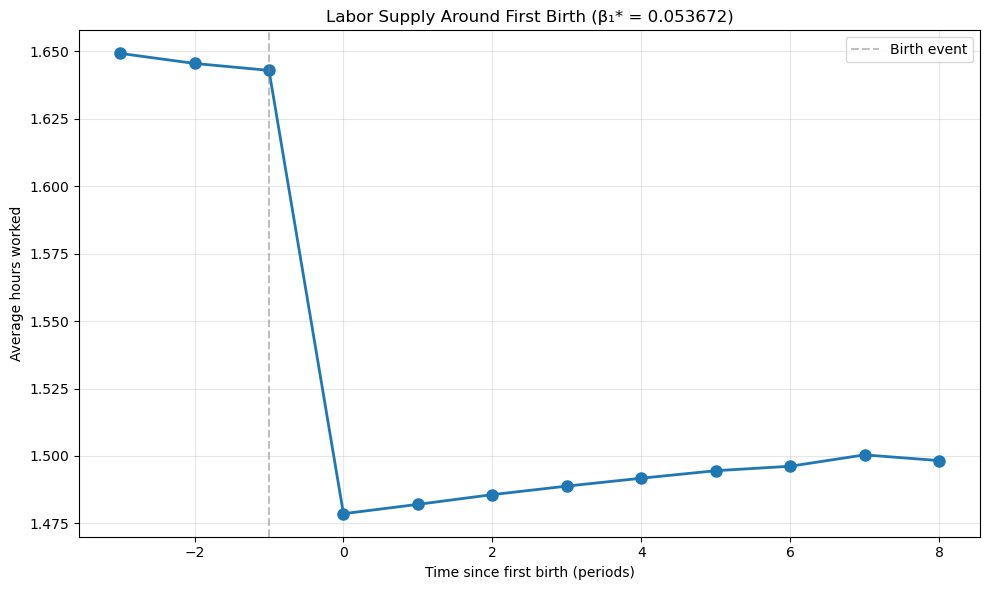
\includegraphics[width=0.5\linewidth]{Billeder/Opgave 1.png}
    \caption{Drop in hours worked from the solved model using the optimised $\beta_1^* = 0.0537$.}
    \label{fig:q1_calibrated}
\end{figure}